\documentclass[oneside,12pt,a4paper]{book}
\usepackage[utf8]{inputenc}
\labelformat{section}{\thechapter.#1}
\usepackage{listings}
\usepackage{FEE}
\pagestyle{CTU_FEE_pagestyle}

%\usepackage{showframe}
\input{acronyms}


\coursename{Algoritmy digitální kartografie a GIS}


\subject{Úloha č. 3:}
\title{Digitální model terénu a jeho analýzy}

\author{Bc. Taťána Bláhová, Bc. Tomáš Krauz, Bc. Adéla Kučerová}


\date{\today} % keep commented to add current date, empty for no date, input version of file (preferred)
\lstset{ 
showstringspaces=false, 
numbers=left, 
numberstyle=\ttfamily\small, 
stepnumber=1, 
firstnumber=last, 
breaklines=T} 




\begin{document}
% \let\cleardoublepage\clearpage
\maketitle

    \vspace{-2cm}
    \vfill
    \begingroup
    
    \tableofcontents
    % \printacronyms
    \vspace{-0.5cm}
    \printglossary[type=\acronymtype,title=\Large Acronyms]
    \endgroup
    \vspace{-1cm}
% \chapter{Example}
% \input{example.tex}


\clearpage
\chapter{Zadání}

\begin{figure}[ht!]
    \centering
    \includegraphics[width=17cm]{fig/zadani_DMT.PNG}
    \caption{Zadání úlohy}
    \label{fig:Zadání úlohy}
\end{figure}



\chapter{Bonusové úlohy} 
\begin{enumerate}
    \item \emph{Triangulace nekonvexní oblasti zadané polygonem. +5b}
    \item \emph{Výběr barevných stupnic při vizualizaci sklonu a expozice. +3b}
    \item \emph{Automatický popis vrstevnic.    +3b}
    \item \emph{Automatický popis vrstevnic respektující kartografické zásady (orientace, shodné rozložení)     +10b}
    \item \emph{Algoritmus pro automatické generování terénních tvarů (kupa, údolí, spočinek, hřbet,...)       +10b}
    \item \emph{3D vizualizace terénu s využitím promítání. +10b}
    \item \emph{Barevná hypsometrie.    +5b}
\end{enumerate}


\chapter{Popis a rozbor problému} 
Na vstupu je množina bodů \emph{$P\{p_i\}^n_{i=0}$}, kde jednomu bodu náleží trojice souřadnic [x,y,z].
Úkolem je pak vytvořit Delaunayho triangulaci (dále jen 'DT'), která je tvořena trojúhelníky \emph{$t_j$}. Stejné trojúhelníky jsou použity i pro další analýzy terénu.\par
K výpočtu bylo využito \cite{dmt}

\section{Delaunayho triangulace}
Výsledkem DT je množina trojúhelníků, které se svým tvarem přibližují rovnostranným trojúhelníkům. Triangulace má čtyři základní vlastnosti: v kružnici opsané trojúhelníku neleží žádný další bod, je maximalizován minimální úhel (nedochází k minimalizaci max. úhlu v trojúhelníku), je lokálně i globálně optimální vůči kritériu minimálního úhlu, je jednoznačná, pokud nebudou čtyři body na jedné kružnici.

\section{Lineární interpolace vrstevnic}
Trojúhelník je tvořen třemi hranami ($e_1$, $e_2$, $e_3$). Je řešen případ vodorovné roviny a jejího průniku s hranami trojúhelníku. Přičemž mohou nastat tři stavy:
\begin{enumerate}
    \item ($z-z_i$)($z-z_{i+1}$) $<$ 0 \longrightarrow $e_i$ protíná vodorovnou rovinu o urč. výšce
    \item ($z-z_i$)($z-z_{i+1}$) $>$ 0 \longrightarrow $e_i$ neprotíná vodorovnou rovinu o urč. výšce
    \item ($z-z_i$)($z-z_{i+1}$) $=$ 0 \longrightarrow $e_i$ leží ve vodorovné rovině o urč. výšce
\end{enumerate}

Pro případ 1) jsou pak spočteny polohové souřadnice X a Y. Souřadnice Z je známa jako výška vodorovné roviny.
\begin{equation}
    x = \frac{(x_2 - x_1)(z-z_1)}{z_2-z_1}+x_1
\end{equation}
\begin{equation}
    y = \frac{(y_2 - y_1)(z-z_1)}{z_2-z_1}+y_1
\end{equation}

\section{Expozice}
Expozicí se rozumí orientace trojúhelníku, která je dána azimutem průmětu gradientu $\nabla \rho$ do roviny x,y. Azimut je určen podle vzorce $A = arctan (n/m)$, kde m a n jsou vektorové součiny pro vektory $\Vec{u}$ a $\Vec{v}$.\par
Hodnota azimutu byla převedena na interval od 0 do $2\pi$ a transformována na interval barvy od 0 do 255. Převod na interval barvy byl proveden kvůli plynulému navázání azimutů blízkých nule a azimutů blízkých 360°. Bylo tak získáno osvětlení terénu od severního směru.\par
Barva slouží k vizualizaci expozice.\par

\section{Sklon}
Sklonem je chápán úhel mezi svislicí a normálou trojúhelníku. Sklon je určen vztahem:\par
\begin{equation}
    \phi = arccos(\frac{\Vec{n}*\Vec{n_t}}{|\Vec{n}||\Vec{n_t}|})
\end{equation}
kde $\Vec{n} = (0,0,1)$ a $\Vec{n_t}=\Vec{u} \times \Vec{v}$.\par

Ze všech trojúhelníků byly vybrány minimální a maximální hodnoty sklonů a následujícím vzorcem byla určena korespondující barva:
\begin{equation}
    barva =(slope - minSlope)*\frac{255}{maxSlope-minSlope}
\end{equation}

Hodnota barvy je pak využita k vizualizaci sklonu pomocí černobílé škály (odstíny šedi), kde všechny tři parametry byly rovny hodnotě barva: RGB(barva, barva, barva).


\chapter{Popis použitých algoritmů}
\label{kapitola: Popis použitých algoritmů}

\section{Delaunayova triangulace}
K tvorbě DT byla použita inkrementální konstrukce, kde vybraný Delaunayho bod musí ležet v levé polorovině úsečky s orientací. Poloměr kružnice opsané trojúhelníku je minimální se středem v pravé polorovině hran. Nelze-li takovýto bod nalézt, je otočena orientace této úsečky.\par

Algoritmus$:$
\begin{enumerate}
\item $p_1$=rand(P) // nahodný bod
\item $p_2$= arg $min_{p_i \in P}$ $||$ $p_1$ - $p_i$$||_2$ // nejbližší bod
\item vytvoř hrany e =($p_1$,$p_2$), e' = ($p_2$,$p_1$)
\item $AEL \longleftarrow e, AEL \longleftarrow e'$ // přidání 2 hran do AEL
\item while AEL not empty$:$
\item \quad \quad $e_1$ = AEL.pop(), $e_1$=($p_1$,$p_2$) // vezmi první hranu z AEL
\item \quad \quad $e'_1$ = ($p_2$, $p_1$) // prohoď její orientaci
\item \quad \quad \overline{p} = arg $max_{\forall p_i \in \sigma_L (e'_1)}$ \angle{$p_1$,$p_i$,$p_2$} // najdi Delaynayovský bod
\item \quad \quad if $\exists \overline{p}:$ // takový bod existuje
\item \quad \quad \quad \quad $e_2$=($p_2$,$\overline{p}$), $e_3$=($\overline{p}$, $p_1$) // vytvoř zbývající hrany trojúhelníku
\item \quad \quad \quad \quad $DT \longleftarrow e'_1$, $DT \longleftarrow e_2$, $DT \longleftarrow e_3$ // přidat hrany do $DT$
\item \quad \quad \quad \quad update AEL($e_2$,AEL), add($e_3$,AEL) // Update AEL
\end{enumerate}
Při přidání e = (a,b) do AEL. Kontrola, zda neobsahuje hranu s opačnou orientací e' = (b,a), pokud ano, tak je taková e' odstraněna z AEL. Pokud tam ještě není, je e přidána do AEL. Triangulace je ukládána po trojúhelnících.\par

\begin{enumerate}
\item vytvoř hranu e' =(b,a)
\item if ($e'$ \in AEL)
\item $AEL \longrightarrow e'$, odstran z AEL
\item else

\item $AEL \longleftarrow e,$ pridej do AE
\item $DT \longleftarrow (a,b)$, pridej do DT
\end{enumerate}

%\section{Generování terénních tvarů}
%V aplikaci jsou implementovány tři druhy terénních tvarů: kupa, hřbet a sedlo.\par

%\subsection{Kupa}
%Pro výpočet kupy byl využit tvar tzv. rotačního paraboloidu
%\begin{equation}
%    \mathrm{z = -(x_i - x_t)^2 - (y_i - y_t)^2}
%\end{equation}
%kde hodnoty s indexem t jsou souřadnice těžiště všech bodů.\par

%\subsection{Hřbet}
%Tvar pro typ hřbet byl vegenerován rovnicí$:$
%\begin{equation}
%    \mathrm{z = \sqrt{y^2_t - (y_i - y_t)^2} + x_i}
%\end{equation}


%\subsection{Sedlo}
%%Tvar sedla byl vygenerován následující rovnicí$:$
%\begin{equation}
%    \mathrm{z = (x_i - x_t)^2(y_i-y_t)^2}
%\end{equation}

%\subsection{Implementace}
Implementování bylo provedeno tak, že v prvním kroce bylo vygenerováno n bodů o náhodných souřadnicích polohy x, y, aby se vešly do vykreslovacího okna Canvas. Dále byly spočteny souřadnice těžiště. Byl počítán cyklus FOR pro n bodů, kde souřadnice Z byly vypočteny pomocí výše uvedených rovnic pro kupu, hřbet a sedlo.\par

\section{Generování vrstevnic a jejich popisů}
Po vytvoření DT nad daty, je možné v dalším zpracování - tedy generování vrstevnic. Vrstevnice (izohypsy) jsou linie spojující místa se stejnou předem určenou nadmořskou výškou.\par

\subsection{Generování vrstevnic}
Předpokladem je již mít trojúhelníkovou síť. Hlavní vrstevnice jsou zobrazeny výraznější linií, než jsou vedlejší vrstevnice.

Algoritmus pro získání vrstevnic$:$
Vstupem je DT.
\begin{enumerate}
\item Pro $t_j \in DT$, kde $t_j = (e_{j.i}, e_{(j.i)+1}, e_{(j.i)+2})$
\item {$dz_{i1}$= $z_{j1}-z$},
\item {$dz_{i2}$= $z_{j2}-z$},
\item {$dz_{i3}$= $z_{j3}-z$}, vyskove rozdily
\item {$dz_{i12}$= $z_{j1}*z_{j2}$},
\item {$dz_{i23}$= $z_{j2}*z_{j3}$},
\item {$dz_{i31}$= $z_{j3}*z_{j1}$}, souciny vyskovych rozdilu
\item {$if(dz_{i1}=0) \&\& (dz_{i2}=0) \&\& (dz_{i3}=0)$}, komplanarita rovin
\item \quad Continue
\item {else if $(dz_{j1}==0) \&\& (dz_{j2}==0)$}
\item \quad {$Contours \longleftarrow e_{ji}$}, pridej do vrstevnic
\item {else if $(dz_{j2}==0) \&\& (dz_{j3}==0)$}
\item \quad {$Contours \longleftarrow e_{(ji)+1}$}, pridej do vrstevnic
\item {else if $(dz_{j3}==0) \&\& (dz_{j1}==0)$}
\item \quad {$Contours \longleftarrow e_{(ji)+2}$}, pridej do vrstevnic
\item {else if $((dz_{j12}<=0))\&\&(dz_{j23}<0)$ $||$ $((dz_{j12}<0)\&\&(dz_{j23}<=0))$}
\item \quad {$A = getContourPoint(p_{j1},p_{j2},z)$}
\item \quad {$B = getContourPoint(p_{j2},p_{j3},z)$}
\item \quad {$Contours \longleftarrow e(A,B)$}, pridej do vrstevnic
\item {else if $((dz_{j23}<=0))\&\&(dz_{j31}<0)$ $||$ $((dz_{j23}<0)\&\&(dz_{j31}<=0))$}
\item \quad {$A = getContourPoint(p_{j2},p_{j3},z)$}
\item \quad {$B = getContourPoint(p_{j3},p_{j1},z)$}
\item \quad {$Contours \longleftarrow e(A,B)$}, pridej do vrstevnic
\item {else if $((dz_{j31}<=0))\&\&(dz_{j12}<0)$ $||$ $((dz_{j31}<0)\&\&(dz_{j12}<=0))$}
\item \quad {$A = getContourPoint(p_{j3},p_{j1},z)$}
\item \quad {$B = getContourPoint(p_{j1},p_{j2},z)$}
\item \quad {$Contours \longleftarrow e(A,B)$}, pridej do vrstevnic
\end{enumerate}

Algoritmus pro získání bodů vrstevnic$:$
Vstupem dva body se souřadnicemi x a y.
\begin{enumerate}
    \item {$x=\frac{(x_2-x_1)(z-z_1)}{(z_2-z_1)}+x_1$}
    \item {$y=\frac{(y_2-y_1)(z-z_1)}{(z_2-z_1)}+y_1$}
\end{enumerate}

Algoritmus pro získání hlavních vrstevnic$:$
Vstupem jsou vrstevnice, kde každá k-tá vrstevnice je hlavní s výškovým intervalem dz.
\begin{enumerate}
    \item $dh = dz * k$
    \item for e \in Contours
    \item \quad {$z = getZ(e)$}, ziskej vysku hrany
    \item \quad if {$z\%dh ==0$}, zbytek po deleni
    \item \quad \quad $ContoursMain \longleftarrow pair<z,e>$, pridej hranu s vyskou jako par do struktury
\end{enumerate}


%\chapter{Problematické situace a jejich rozbor} 

%\section{DOPSAT}
%DOPSAT.

%\section{DOPSAT}
%\subsection{XXX}
%DOPSAT


%\subsection{XXX}
%XXXXX


\chapter{Vzhled aplikace}
%% nutno dopsat
Po spuštění aplikace se zobrazí následující okno, zde je možnost si vybrat z menu. Menu obsahuje načtení csv souboru, konec aplikace, výpočet DT, vytvoření vrstevnic, analýza sklonu nebo orientace. Dále je zde nastavení vrstevnic (interval, minimální a maximální vrstevnici) a tlačítko na vymazání celého obsahu.
\begin{figure}[ht!]
    \centering
    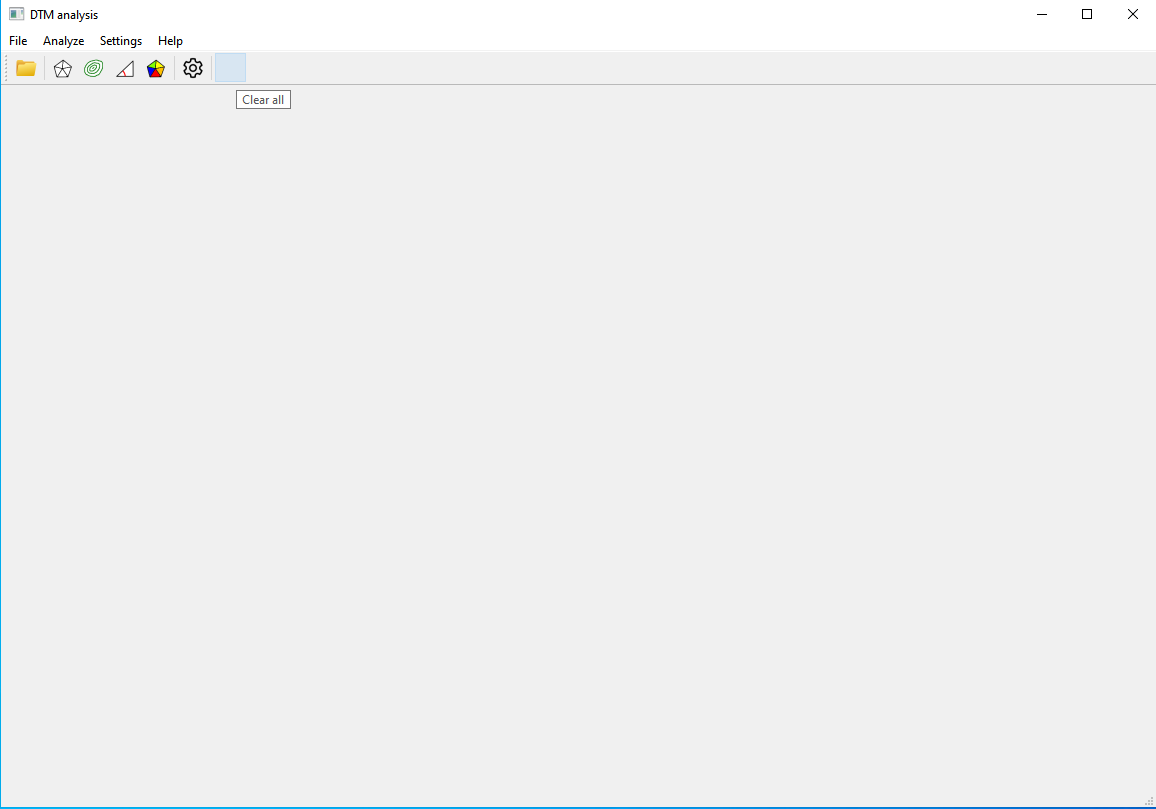
\includegraphics[width=\linewidth]{fig/vzhled.PNG}
    \caption{Vzhled aplikace}
    \label{fig:Zadání úlohy}
\end{figure}

\begin{figure}[ht!]
    \centering
    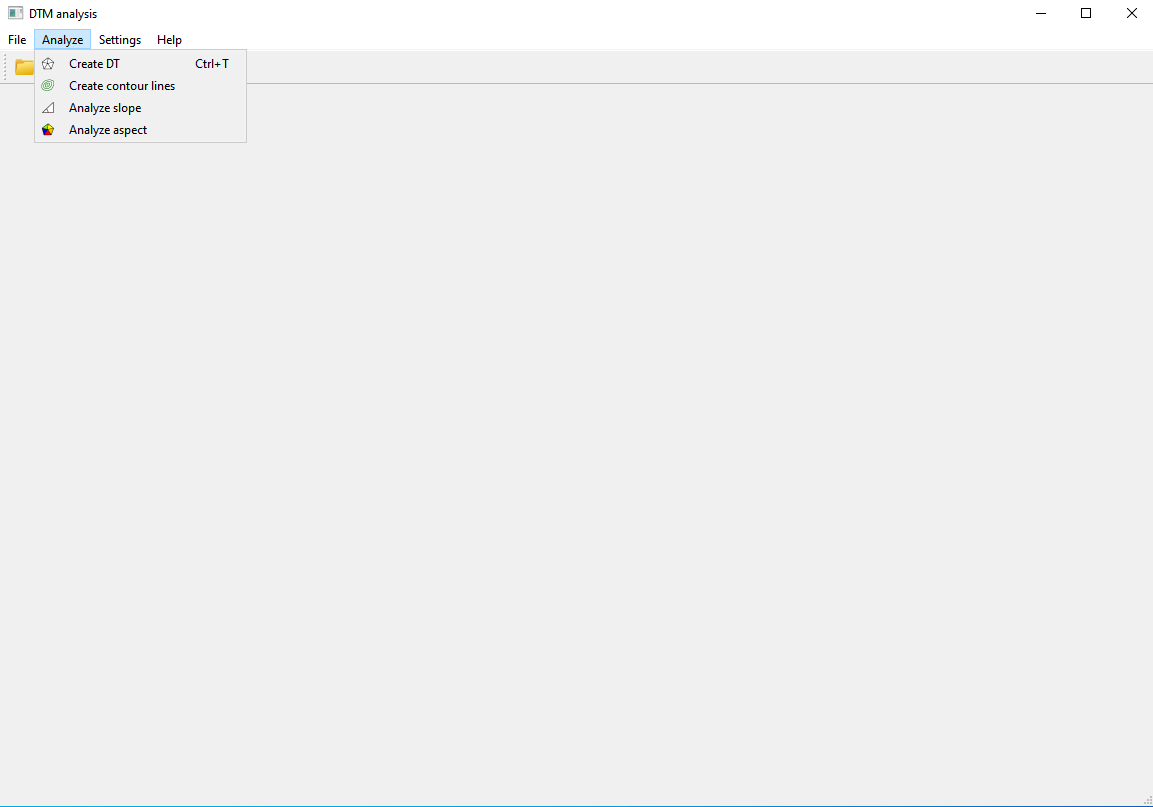
\includegraphics[width=\linewidth]{fig/vzhled2.PNG}
    \caption{Menu aplikace}
    \label{fig:Zadání úlohy22}
\end{figure}

\chapter{Vstupní data} 
Vstupní data je možno vložit 2 způsoby. 
\begin{enumerate}
    \item Naklikat body v programu
    \item Pomocí tlačítka Open otevřít csv soubor.
\end{enumerate}

\section{Vložení bodů pomocí kliknutí myší}

Prvním způsobem, jak vygenerovat body do aplikace, je pomocí kliknutí, kdy je vygenerována souřadnice s náhodnou Z souřadnicí v rozmezí <0,1000>.

\section{Načtení bodů ze csv souboru}
Načtení bodů pomocí csv souboru je možno po kliknutí na tlačítko open. Otevře se vyhledávací okno a je možno si načíst libovolný csv soubor s mračnem bodu. Soubor csv vypadá následovně podle obrázku \ref{fig:csv}. Kde jsou body vloženy v pořadí ID, X, Y, Z. Důležité je, aby soubor měl hlavičku a oddělovač byl pomocí čárky.

\begin{figure}[ht!]
    \centering
    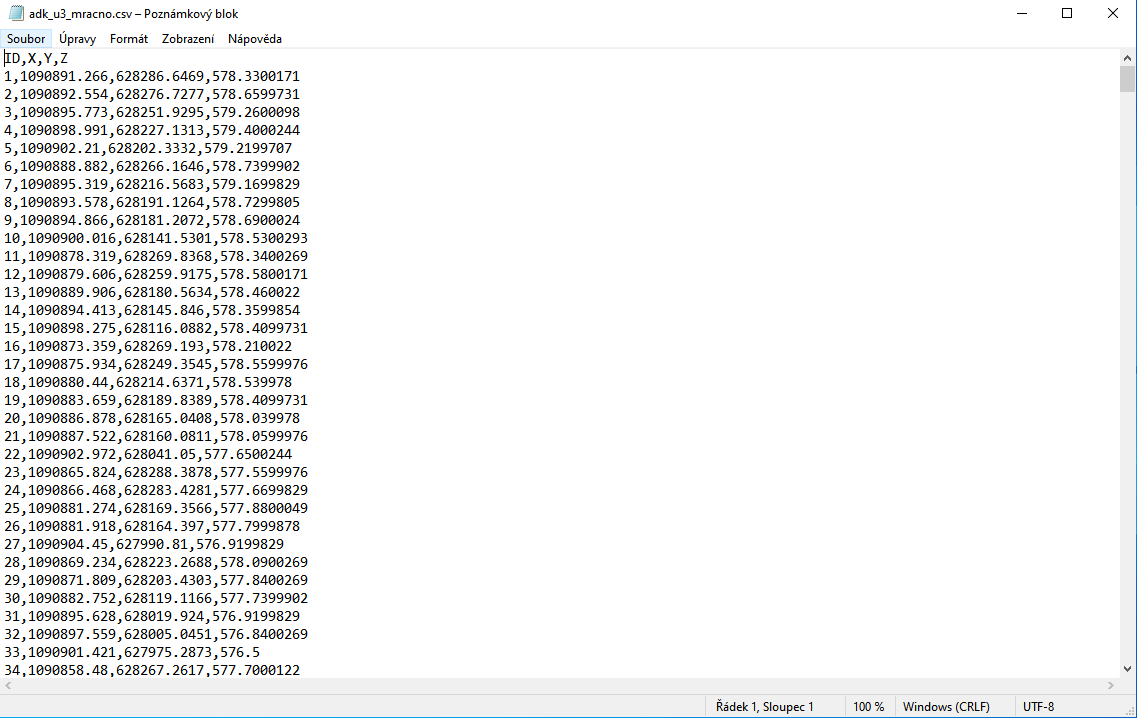
\includegraphics[width=\linewidth]{fig/csv_Data.PNG}
    \caption{csv soubor}
    \label{fig:csv}
\end{figure}

\chapter{Výstupní data} 
Po načtení dat nebo vytvoření dat, je možno vytvořit DT a následně i vytvořit vrstevnice podle zadaného intervalu. Je možné vytvořit sklon či expozici z dat. Poté je možné aplikaci ukončit.

\begin{figure}[ht!]
    \centering
    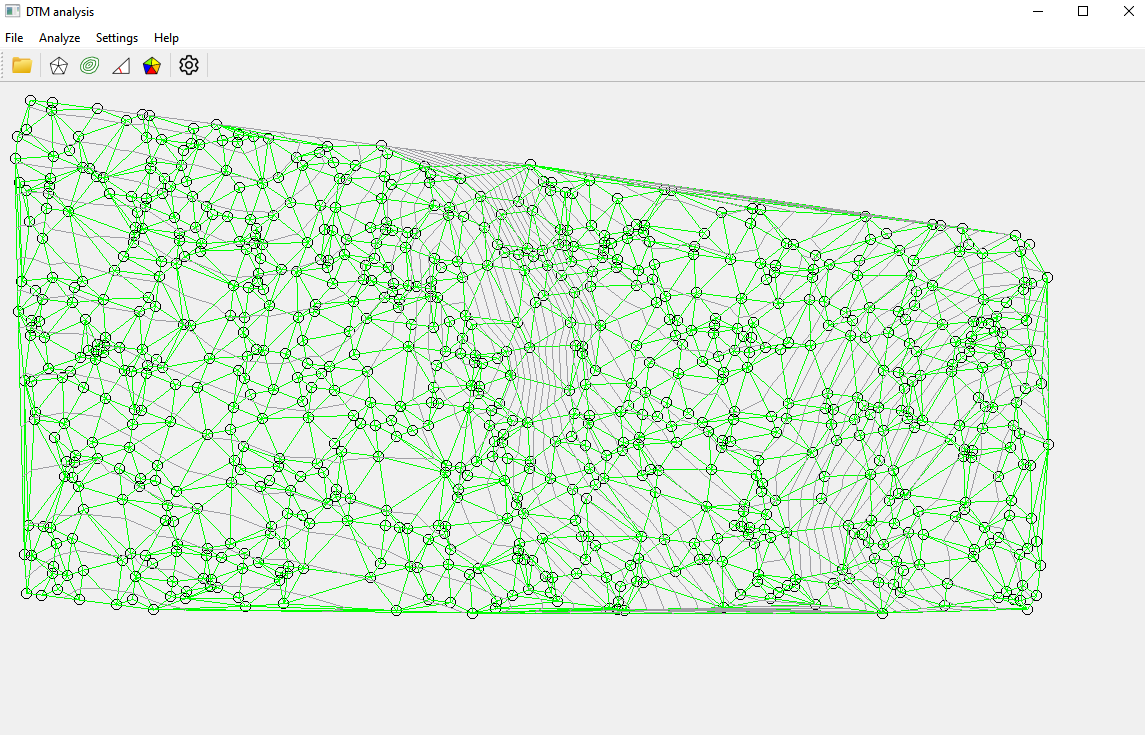
\includegraphics[width=\linewidth]{fig/DT_vrstevnice.PNG}
    \caption{Načtení csv souboru, následně vytvořené DT společně s vrstevnicemi.}
    \label{fig:csv}
\end{figure}

\begin{figure}[ht!]
    \centering
    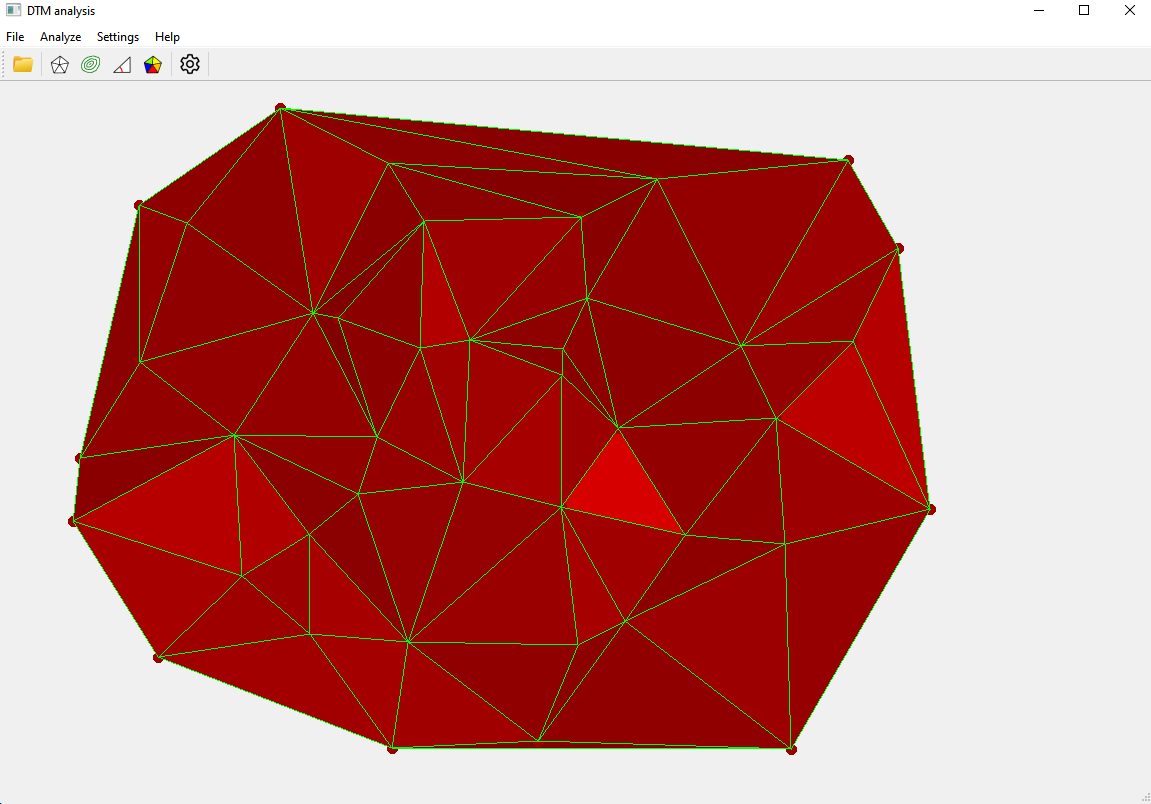
\includegraphics[width=\linewidth]{fig/slope_bez_vrst.PNG}
    \caption{Vytvoření sklonu bez vrstevnic.}
    \label{fig:csv}
\end{figure}

\chapter{Problematické situace a jejich rozbor}
Delaunyho triangulace dává dobré výsledky pro terény, které jsou hladké a spojité, takže u skalních převisů, liniových staveb a lidských úprav terénu nemusí aplikace dávat dobré výsledky. 
Samotná aplikace má v sobě mouchy, není vidět ikona pro vyčistění aplikace. Dále byla vytvořena funkce pro orientaci terénu, která funguje, nicméně se nechce vykreslit.

\chapter{Dokumentace} 
\section{Třída Algorithms}
    \begin{itemize}
    \item $int \;getPointLinePosition(const QPoint3D \; \&p1, const QPoint3D\;\&p2,const QPoint3D \;\&q)$
    \begin{itemize}
    \item analyzuje vzájemný vztah bodu a přímky
    \end{itemize}
    \item $double\; getTwoLinesAngle(const QPoint3D \; \&p1,const QPoint3D \; \&p2,const QPoint3D \; \&p3,const QPoint3D \; \&p4)$
        \begin{itemize}
    \item vypočítá úhel mezi dvěma vektory
    \end{itemize}
    \item $int\; getNearestPoint(const QPoint3D \; \&p, const std::vector<QPoint3D> \; \&points)$
        \begin{itemize}
    \item vrací index nejbližšího bodu k bodu p
    \end{itemize}
    \item $int\; getDelaunayPoint(const QPoint3D \;\&p1, const QPoint3D\; \&p2,const std::vector<QPoint3D>\; \&points);$
        \begin{itemize}
    \item vrací index Delaunayho bodu v rámci vektoru bodů
    \end{itemize}
    \item $std::vector<Edge>\; createDT(const\; std::vector<QPoint3D>\; &points);$
        \begin{itemize}
    \item vytvoří DT ze vstupních bodů
    \end{itemize}
    \item $void updateAEL\;(const\; Edge\; \&e, std::list<Edge>\; \&ael);$
        \begin{itemize}
    \item aktualizuje hranu v listu hran
    \end{itemize}
      \item $std::vector<Edge>\; createContourLines\;(const\; std::vector<Edge>\; &dt,\; double\; zmin,\; double\; zmax,\; double\; dz);$
    \begin{itemize}
    \item vrací hrany vrstevnic
    \end{itemize}
    \item $double\; computeSlope\;(const\; QPoint3D\; \&p1, const QPoint3D\; \&p2, const\; QPoint3D\; \&p3);$
        \begin{itemize}
    \item pomocný výpočet pro sklon
    \end{itemize}
    \item $std::vector<Triangle>\; analyzeSlope\;(const\; std::vector<Edge>\; \&dt)$
        \begin{itemize}
    \item vrací hodnotu sklonu trojúhelníku
    \end{itemize}
    \item $double\; computeAspect(const\; QPoint3D \&p1\;, const\; QPoint3D\; \&p2,const\; QPoint3D\; \&p3)$
        \begin{itemize}
    \item pomocný výpočet pro orientaci
    \end{itemize}
    \item $std::vector<Triangle>\; analyzeAspect(const\; std::vector<Edge>\; \&dt)$
        \begin{itemize}
    \item vrátí hodnotu orientace trojúhelníku
    \end{itemize}
\end{itemize}

   \section{Třída Draw} 
    \begin{itemize}
    \item $void\; mousePressEvent(QMouseEvent *event)$
    \begin{itemize}
    \item vrátí souřadnice kurzoru po kliknutí na Canvas
    \end{itemize}
    \item $void\; paintEvent(QPaintEvent *event)$
    \begin{itemize}
    \item vykreslí body na Canvas
    \end{itemize}
        \item $void\; clearContours()$
    \begin{itemize}
    \item vyčistí vrstevnice
        \end{itemize}
    \item $void\; clearPoints()$
    \begin{itemize}
    \item vyčistí body
    \end{itemize}
            \item $void\; clearDT()$
    \begin{itemize}
    \item vyčistí DT
    \end{itemize}
\end{itemize}

   \section{Třída CSV}
    \begin{itemize}
    \item $static\; std::vector<std::vector<std::string>>\; read_csv(std::string\; \&filename);$
    \begin{itemize}
\item načte vstupní csv soubor
\end{itemize}
\item $static\; std::vector<QPoint3D>\; getPoints3D(std::vector<std::vector<std::string>>\; \&csv_content, double\; \&x_min,double\; \&x_max, double\; \&y_min, double\; \&y_max);$
\begin{itemize}
\item vrací vektor QPoint3D z csv souboru
\end{itemize}
\end{itemize}

   \section{Třída Mainform}
    \begin{itemize}
    \item $void \;on\_actionOpen\_triggered()$
    \begin{itemize}
\item otevře průzkumníka souborů
\end{itemize}
    \item $void \;on\_actionCreate\_DT\_triggered()$
    \begin{itemize}
\item vytvoří DT
\end{itemize}
    \item $void \;on\_actionClear\_all\_triggered()$
    \begin{itemize}
\item vyčistí Canvas
\end{itemize}
    \item $void \;on\_actionExit\_triggered()$
    \begin{itemize}
\item ukončí soubor
\end{itemize}
    \item $void \;on\_actionCreate\_contour\_lines\_triggered()$
    \begin{itemize}
\item vytvoří vrstevnice
\end{itemize}
    \item $void \;on\_actionCreate\_slope\_triggered()$
    \begin{itemize}
\item vytvoří sklon svahu
\end{itemize}
    \item $void \;on\_actionCreate\_aspect\_triggered()$
    \begin{itemize}
\item vytvoří orientaci svahu
\end{itemize}
\end{itemize}
\chapter{Závěr} 
Byla vytvořena aplikace pro zpracování množiny bodů, kde výstupem je vytvoření digitálního modelu terénu a analýzy tohoto modelu.

\begingroup
    \pageclear
    \printbibliography[title=Literatura]
\endgroup

% \begingroup
%     \let\clearpage\relax
%     \printbibliography[title=References]
% \endgroup

\end{document}